\documentclass[class=minimal,border=0pt]{standalone}

\usepackage{tudfonts}

\usepackage{tikz}
\usetikzlibrary{calc}
\usetikzlibrary{matrix}
\usetikzlibrary{positioning}

\begin{document}

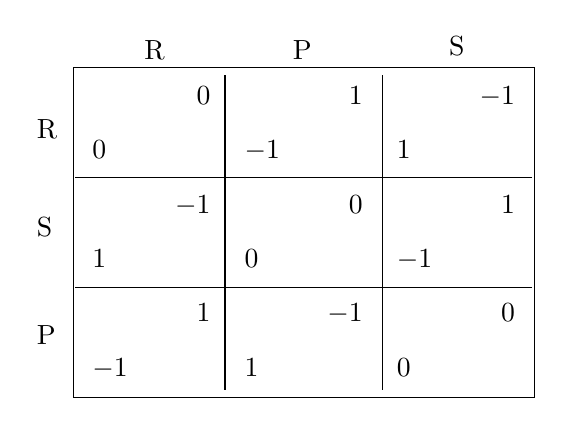
\begin{tikzpicture}

\matrix[matrix of math nodes,every odd row/.style={align=right},every even row/.style={align=left},every node/.style={text width=1.5cm},row sep=0.2cm,column sep=0.2cm] (m) {
$0$&$1$&$-1$\\
$0$&$-1$&$1$\\
$-1$&$0$&$1$\\
$1$&$0$&$-1$\\
$1$&$-1$&$0$\\
$-1$&$1$&$0$\\
};
\draw (m.north east) rectangle (m.south west);
\draw (1,2) -- (1,-2);
\draw (-1,2) -- (-1,-2);
\draw (2.9,0.7) -- (-2.9,0.7);
\draw (2.9,-0.7) -- (-2.9,-0.7);



\coordinate (a) at ($(-3.5,2)!0.25!(m.north east)$);
\coordinate (b) at ($(-1,2)!0.75!(m.north east)$);
\coordinate (e) at ($(-1,2)!0.25!(m.north east)$);
\node[above=5pt of a,anchor=base] {R};
\node[above=5pt of b,anchor=base] {S};
\node[above=5pt of e,anchor=base] {P};

\coordinate (c) at ($(m.north west)!0.25!(-2,-1)$);
\coordinate (d) at ($(m.north west)!0.25!(-2,-6)$);
\coordinate (f) at ($(m.north west)!0.25!(-2,-11.5)$);
\node[left=2pt of c,text width=.5cm]  {R};
\node[left=2pt of d,text width=.5cm]  {S};
\node[left=2pt of f,text width=.5cm]  {P};


\end{tikzpicture}

\end{document}
